\chapter{Used technologies}
\label{chapter:AutoTechnologies}

The technologies used in this thesis are basically the same as in
the first part (see Chapter \ref{chapter:ConfTechnology}).

\section{Eclipse WorkbenchJob API}
\label{section:AutoTechJob}
Since we don't want the UI to block while we are doing our automated
execution run we will use the Eclipse Job API to run our
automated execution thread.
The Job API is specifically designed to accommodate very long running
tasks which makes it perfect for our purposes since an execution
run with several model files and hundreds of trace files might
a whole night.
An example for the use of jobs in the normal Eclipse architecture
is the SVN commit operation seen in Figure \ref{fig:SVNCommit}.

\begin{figure}[SVNCommit]
  \centering
  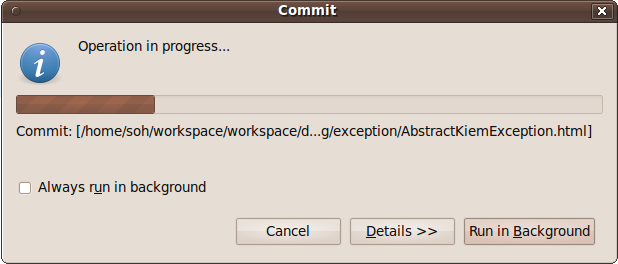
\includegraphics[scale=.4]{SVNCommit.png}
  \caption[The SVN commit job]%
  {The SVN commit job\protect\footnotemark}
  \label{fig:SVNCommit}
\end{figure}



\section{Eclipse Wizards}
\label{section:AutoTechWizards}
To allow the user to set up the execution run we will be using the
Eclipse Wizard API.
Wizards are used to guide the user through the process of creating complex items by taking
the information in a structured way and then generating the item from it.
One example inside the Eclipse Architecture is the Java Class Creation Wizard (see Figure \ref{fig:ClassWizard})
In theory it is possible to just open a text file and enter all the information manually.
However if the wizard is used the user only has to select the class he wants to extend
and the interfaces he wants to implement, activate one check box and then the wizard will
create the class body, all required methods and comments for each element (see Listing \ref{fig:classCreationGenerated})
This makes it very easy for even inexperienced users to create new classes without knowing
the exact syntax.

\begin{figure}[ClassWizard]
  \centering
  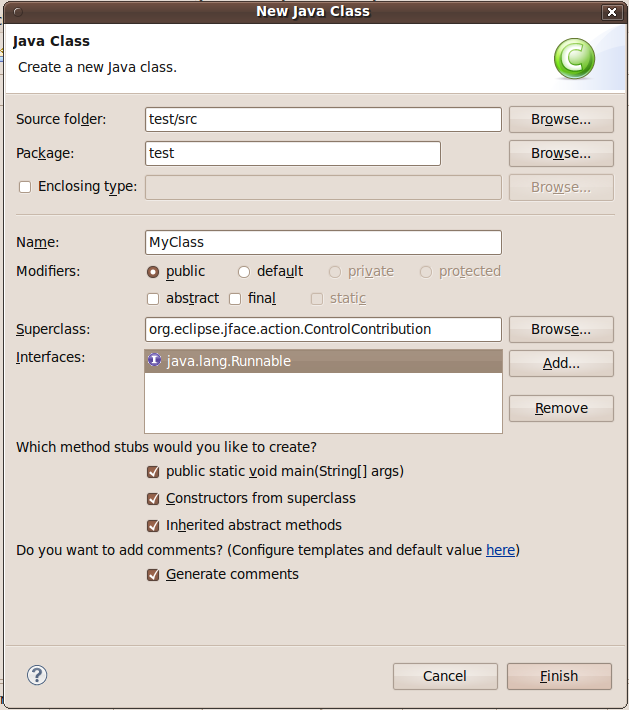
\includegraphics[scale=.4]{ClassWizard.png}
  \caption[The Class Creation Wizard]%
  {The Class Creation Wizard\protect\footnotemark}
  \label{fig:ClassWizard}
\end{figure}

\lstset{
  language=Java,
}
\begin{lstlisting}[caption={Code generated by the wizard},label={fig:classCreationGenerated}]
package test;

import org.eclipse.jface.action.ControlContribution;
import org.eclipse.swt.widgets.Composite;
import org.eclipse.swt.widgets.Control;

/**
 * @author soh
 */
public class MyClass extends ControlContribution implements Runnable {

    /**
     * Creates a new MyClass.java.
     * 
     * @param id
     */
    public MyClass(String id) {
        super(id);
    }

    /**
     * {@inheritDoc}
     */
    @Override
    protected Control createControl(Composite parent) {
        return null;
    }

    /**
     * {@inheritDoc}
     */
    public void run() {
    }

    /**
     * @param args
     */
    public static void main(String[] args) {

    }
}
\end{lstlisting}


